\documentclass[12pt]{article}
\usepackage[top=5mm,includehead,headheight=63pt, left=2.5cm,bottom=2.5cm,right=2.5cm,headsep=0.3cm]{geometry} 
\usepackage{fontspec}
\setmainfont[
 Path = fonts/,
 BoldFont={Veleka-Bold.otf}, 
 ItalicFont={Veleka-Italic.otf},
 BoldItalicFont={Veleka-BoldItalic.otf}
 ]{Veleka-Regular.otf}


%% bibliography packages
\usepackage{biblatex} 
\addbibresource{biblo.bib} 

%%charset packages
\usepackage[utf8]{inputenc}
\usepackage[english,bulgarian]{babel}
\usepackage{textgreek}
\usepackage{textcomp}
\usepackage[T2A]{fontenc}

%% hyperlinks
\usepackage{hyperref}
\usepackage{url}[hyphens]

%% graphics packages
\usepackage{caption}
\usepackage{graphicx}
\usepackage{subfigure}
\graphicspath{{imgs/}}
\usepackage{float}




%%Autoref language settings begin
\renewcommand*{\figureautorefname}{Фиг.}
\renewcommand*{\equationautorefname}{Уравн.}
\renewcommand*{\subsectionautorefname}{Пар.}
\renewcommand*{\subsubsectionautorefname}{\subsectionautorefname}
\newcommand{\subfigureautorefname}{\figureautorefname}
%%Autoref language settings end

%%other
\usepackage[inline]{enumitem}
\usepackage{amsmath}
\usepackage{amssymb}
\usepackage{breqn}
\allowdisplaybreaks
\usepackage{fancyhdr}
\usepackage{afterpage}
\usepackage{listings}
\lstloadlanguages{[5.2]Mathematica}


\title{Математически модел на идеален контакт}
\author{Васил Иванов}
\date{\today}

%%header definitions
\pagestyle{fancy}
\fancyhf{}
\lhead{
\includegraphics[width=0.1\linewidth]{su-logo.png}}
\chead{СОФИЙСКИ УНИВЕРСИТЕТ „Св. КЛИМЕНТ ОХРИДСКИ”\\Факултет по математика и информатика}
\fancyfoot[C]{\ifnum\thepage<2\relax\else\thepage\fi}
%%end header definitions

\begin{document}
\begin{titlepage}
    \thispagestyle{fancy}
    \begin{center}
        \hfill \break
        \hfill \break
        \hfill \break
        \Huge	
        \textbf{Курсова работа}\\
        \vspace{3cm}
    \end{center}
    \normalsize	
    \textbf{\underline{Тема:}} Модел на идеален топлинен контакт
    \vspace{2cm}

    \begin{flushright}
        \normalsize	
        Изготвил: Васил Василев Иванов,

        Магистърска програма: ,,Изчислителна математика и математическо моделиране``
        \vspace{1cm}

        За курса:

        ,,Математически модели и изчислитен експеримент``
    \end{flushright}

    \vspace*{\fill}
    \begin{center}
        \footnotesize	
        София

         ~2022~г.
    \end{center}
 \end{titlepage}
\setcounter{page}{2}

\section{Задача}
Разглеждаме задачата за идеален топлинен контакт:
\begin{align}
	\frac{\partial u_1}{\partial t} & = \kappa_{1}  \frac{\partial ^ 2 u_1}{\partial x ^ 2}, - \infty < x < 0; 0 < t \leq T \\ 
	\frac{\partial u_2}{\partial t} & = \kappa_{2}  \frac{\partial ^ 2 u_2}{\partial x ^ 2}, 0 < x < \infty; 0 < t \leq T   
\end{align}
Където:
\begin{equation}
	\kappa_{i} = \frac{k_{i}}{\rho_{i} c_{i}}
\end{equation}

\begin{itemize}
	\item $\kappa_{i}$ - температуропроводност
	\item $k_{i}$ - топлопроводност
	\item $c_{i}$ - топлинен капацитет
	\item $\rho_{i}$  - плътност на материала
\end{itemize}

Наложено е и следното прекъснато начално условие
\begin{align}
	u_{1}(x, t = 0) & = 0, -\infty < x < 0  \\
	u_{2}(x, t = 0) & = u_0, 0 < x < \infty 
\end{align}

Както и гранични условия ,,на безкрайност``:
\begin{align}
	u_{1}(-\infty, t) & = 0, t > 0   \\
	u_{2}(+\infty, t) & = u_0, t > 0 
\end{align}
 
И условията за идеален контакт:
\begin{align}
	u_{1}(0, t)                                 & = u_2(0, t),  t > 0                                  \\
	k_{1}\frac{\partial u_1}{\partial x} (0, t) & = k_{2}\frac{\partial u_2}{\partial x} (0, t), t > 0 
\end{align}

Дефинираме и ,,помощна константа`` $\beta$ с цел олекотяване на записа:
\begin{equation*}
	\beta = \frac{\sqrt{k_2 \rho_2 c_2}}{\sqrt{k_1 \rho_1 c_1}}
\end{equation*}

За така поставената задача е известно и точното (аналитично решение):
\begin{align}
	u_{1}(x, t) & = \frac{\beta u_0}{1+\beta} \left[1 + \erf{\left(\frac{2}{2\sqrt{\kappa_1 t}}\right)}\right] \\
	u_{2}(x, t) & = \frac{u_0}{1+\beta} \left[\beta + \erf{\left(\frac{2}{2\sqrt{\kappa_2 t}}\right)}\right]   
\end{align}
Където: 
\begin{equation*}
	\erf{(z)} = \frac{2}{\sqrt{\pi}} \displaystyle\int_{0}^{z} e ^{-t^2} dt
\end{equation*}
За целите на изследването на полученото числено решение ще използваме следните физични пареметри за различни материали:\\
\begin{figure}[h]
	\centering
	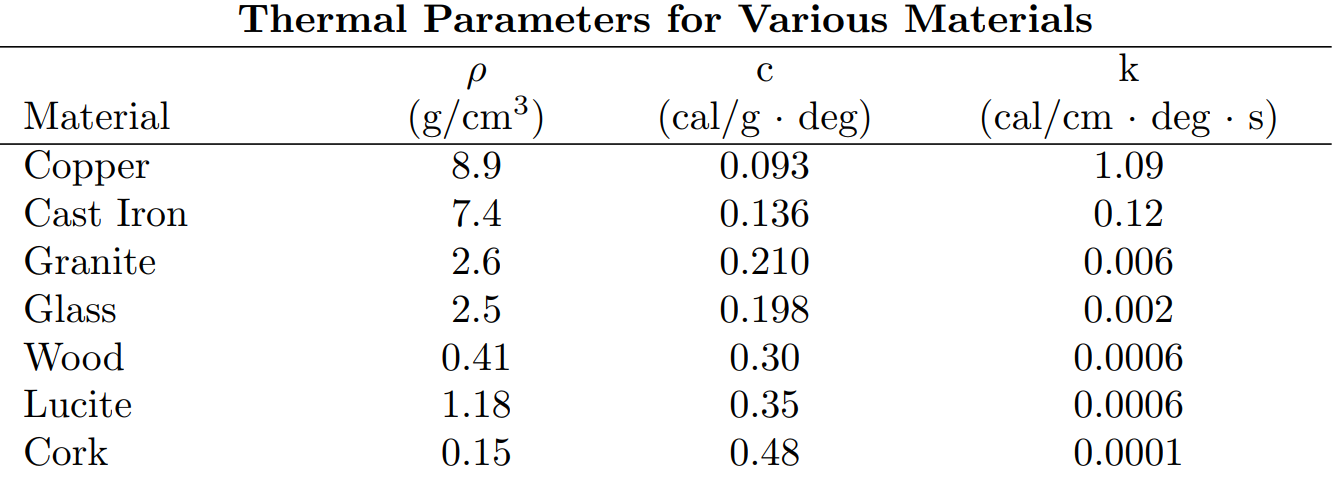
\includegraphics[width=\linewidth]{constants.png}
	\caption{Термофизични константи за различни материали}
	\label{fig:constants}
\end{figure}

\section{Построяване на диференчна схема}
Искаме да построим диференчна схема с втори ред на точност, т.е. $O(h^2 + \tau)$, където $h$ - стъпката на дискретизацията по пространството и $\tau$  - стъпка на дискретизация по времето.
Това условие за грешката създава съответни проблеми, предвид прекъснатото решение в точката на контакт.

\noindent Разглеждаме (точното) решението като една функция $u(x)$:
\begin{equation}
	u(x)=
	\begin{cases}
		u_1(x) & \text{ако } x \in (-\infty, 0) \\
		u_2(x) & \text{ако } x \in [0, +\infty) 
	\end{cases}
\end{equation}
Приближеното решение за $u(x)$ в точката $(x_i, t_j)$ от мрежата ще бележим с $y_{i}^{j}$. ,,Безкрайността`` ще апроксимираме с т.нар. ,,актуална безкрайност``, т.е. ще разглеждаме достатъчно голям интервал $[-M, M]$, за някое положително число $M$.

\noindent Въвеждаме мрежата:
\begin{equation*}
	\omega_{h, \tau } = \left\{ (x_i, t_j):  x_i = -M + (i-1) h, t_j = (j-1) \tau; i = \overline{1,2n+1}, j = \overline{1,m+1};  n = \left\lceil \frac{2M}{h} \right\rceil, m =\left\lceil \frac{T}{\tau} \right\rceil \right\}
\end{equation*}

\noindent Условията за устойчивост на схемата (т.е за $h$ и $\tau$) ще определим след малко.
Да забележим, че при така построената мрежа, на $j$-тия слой по времето, стойността на приближеното решение в точката на котакт ще бъде $y_{n+1}^j$.

Можем вече да апроксираме основните диференциални уравнения. Използваме формулата с разлика напред за производните по времето и формулата с втори ред на точност за втората производна.
С изключение на точките на контакт това е стандартна диференчна схема с грешка $O(h^2+\tau)$ за линейна дифузионна задача. Затова можем директно да запишем:
\begin{align}
	y_{i}^{j+1} & = \left(1-\frac{2 \tau \kappa_1}{h^2}\right)y_{i}^j + \frac{\tau \kappa_1}{h^2}\left(y_{i-1}^j + y_{i+1}^j\right); j = \overline{1, m}; i  = \overline{2, n}    \\
	y_{i}^{j+1} & = \left(1-\frac{2 \tau \kappa_2}{h^2}\right)y_{i}^j + \frac{\tau \kappa_2}{h^2}\left(y_{i-1}^j + y_{i+1}^j\right); j = \overline{1, m}; i  = \overline{n+2, 2n} 
\end{align}
На база тези две диференчни уравнения ще получим и условията за устойчивост на схемата. Избираме:
\begin{align*}
	\tau & < \frac{h^2}{2 d}                         \\
	d    & := max \left\{\kappa_1, \kappa_2 \right\} 
\end{align*}
Остава да апроксираме с втори ред на точност задачата и в особената точка.

За целта ще се върнем към оригиналната дефиниция на задачата и като начало ще апроксираме производните в условието за идеален контакт с формула с  грешка $O(h+\tau)$:
\begin{align*}
	\frac{\partial u_1}{\partial x} (0, t)  & = \frac{k_2}{k_1} \frac{\partial u_2}{\partial x} (0, t)     \\
	\phi_{n+1}^{j}                          & = \psi_{n+1}^{j}                                             \\
	\frac{\phi_{n+1}^{j} - \phi_{n}^{j}}{h} & =  \frac{k_2}{k_1} \frac{\psi_{n+2}^{j} - \psi_{n+1}^{j}}{h} 
\end{align*}
Където $\phi_i^j$ и $\psi_i^j$ са съотвените приближени решения за $u_1(x,t)$ и $u_2(x,t)$.
За безизточниковото уравнение на дифузията при дифузионен коефициент \textbf{1}, лесно се показва чрез развиване в ред на Тейлър и допускане, че основното диференциално уравнение
е изпълнено с достатъчно добра точност и върху границите (съображения за гладкост на решението), че трябва от лявата страна на горното диференчно уравнение да извадим $\frac{\partial u_1}{\partial t}$, a от дясната: $-\frac{k_2}{k_1}\frac{\partial u_2}{\partial t}$.
Дискертизираме производните по времето в тези допълнителни членове с формулата с разлика напред и получаваме:
\begin{align*}
	\phi_{n+1}^{j}                                                                                      & = \psi_{n+1}^{j}                                                                                                          \\
	\left(\frac{\phi_{n+1}^{j} - \phi_{n}^{j}}{h} - \frac{\phi_{n+1}^{j+1}-\phi_{n+1}^{j}}{\tau}\right) & =  \frac{k_2}{k_1} \left(\frac{\psi_{n+2}^{j} - \psi_{n+1}^{j}}{h} + \frac{ \psi_{n+1}^{j+1}-\psi_{n+1}^{j}}{\tau}\right) 
\end{align*}
С помощта на системата \textit{Mathematica} извършваме необходимите алгебрични преобразувания и се връщаме към нотацията на ,,общо`` приближено решение $y_i^j$:
\begin{equation}
	y_{n+1}^{j+1} = \frac{2 \tau}{h^2} \frac{k_1 \kappa_1 \kappa_2 }{\kappa_2 k_1 + \kappa_1 k_2} y_{n+1}^j + \left( 1 - \frac{2 \tau}{h^2}  \frac{(k_1 + k_2) \kappa_1 \kappa_2 }{\kappa_2 k_1 + \kappa_1 k_2} \right) y_{n+1}^j + \frac{2 \tau}{h^2} \frac{k_2 \kappa_1 \kappa_2 }{\kappa_2 k_1 + \kappa_1 k_2} y_{n+2}^j
\end{equation}
Горното е за $j > 1$, т.е. за слоеве по времето след първия (определен от началното условие).
Тогава можем да обобщим всички разсъждения дотук в следната диференчна схема, с която ще получаваме приближеното решение на задачата:
\begin{align*}
	y_i^1          & = 0, i = \overline{1,n}                                                                                                                                                                                                                                                                                   \\
	y_i^{1}        & = u_0, i = \overline{n+1, 2n+1}                                                                                                                                                                                                                                                                           \\
	\\
	За j         & = \overline{1,m+1}:                                                                                                                                                                                                                                                                                       \\
	y_{i}^{j+1}    & = \left(1-\frac{2 \tau \kappa_1}{h^2}\right)y_{i}^j + \frac{\tau \kappa_1}{h^2}\left(y_{i-1}^j + y_{i+1}^j\right);  i  = \overline{2, n}                                                                                                                                                                  \\
	y_{n+1}^{j+1}  & = \frac{2 \tau}{h^2} \frac{k_1 \kappa_1 \kappa_2 }{\kappa_2 k_1 + \kappa_1 k_2} y_{n+1}^j + \left( 1 - \frac{2 \tau}{h^2}  \frac{(k_1 + k_2) \kappa_1 \kappa_2 }{\kappa_2 k_1 + \kappa_1 k_2} \right) y_{n+1}^j + \frac{2 \tau}{h^2} \frac{k_2 \kappa_1 \kappa_2 }{\kappa_2 k_1 + \kappa_1 k_2} y_{n+2}^j \\
	y_{i}^{j+1}    & = \left(1-\frac{2 \tau \kappa_2}{h^2}\right)y_{i}^j + \frac{\tau \kappa_2}{h^2}\left(y_{i-1}^j + y_{i+1}^j\right);  i  = \overline{n+2, 2n}                                                                                                                                                               \\
	y_{1}^{j+1}    & = 0                                                                                                                                                                                                                                                                                                       \\
	y_{2n+1}^{j+1} & = u_0                                                                                                                                                                                                                                                                                                     \\
\end{align*}

Така написаната диференчна схема може директно да бъде инплементирана например в \textit{Mathematica}. Кодът използван за следващите числени експерименти може да бъден намерен във файла \textit{mmieproj-code.nb}.
\end{document}
